\section{When Does Data Sharing Actually Help in Offline Multi-Task RL?}
\label{sec:analysis}

% Since offline RL algorithms bear the promise of converting large logged datasets into effective and generalizing behaviors, a natural use-case of offline RL are situations where we have access to large pool of data from a number of tasks and scenarios. 
Our goal is to leverage experience from all tasks to learn a policy for a particular task of interest. Perhaps the simplest approach to leveraging experience across tasks is to train the task policy on not just the data coming from that task, but also relabeled data from all other tasks~\citep{caruana1997multitask}.
%%AK: I want to add a citation here, but I dont want to cite more advanced methods that relabel based on optimality since this is not quite the focus of this sentence, what should I cite?
%%TY.5.27: I cited the 1997 paper. Not sure if it is the most appropriate one though.
Is this na\"ive data sharing strategy sufficient for learning effective behaviors from multi-task offline data? In this section, we aim to answer this question via empirical analysis on a relatively simple domain, which will reveal interesting aspects of data sharing. We first describe the experimental setup and then discuss the results and possible explanations for the observed behavior. Using insights obtained from this analysis, we will then derive a simple and effective data sharing strategy in Section~\ref{sec:method}.

\textbf{Experimental analysis setup.} To assess the efficacy of data sharing, we experimentally analyze various multi-task RL scenarios created with the walker2d environment in Gym~\citep{brockman2016openai}. We construct different test scenarios on this environment that mimic practical situations, including settings where different amounts of  data of varied quality are available for different tasks~\citep{kalashnikov2021mt,xie2019improvisation,singh2020parrot}. In all these scenarios, the agent attempts three tasks: \texttt{run forward}, \texttt{run backward}, and \texttt{jump}, which we visualize in Figure~\ref{fig:env}. Following the problem statement in Section~\ref{sec:prelims}, these tasks share the same state-action space and transition dynamics, differing only in the reward function that the agent is trying to optimize. 
Different scenarios are generated with varying size offline datasets, each collected with policies that have different degrees of suboptimality. This might include, for each task, a single policy with mediocre or expert performance, or a mixture of policies given by the initial part of the replay buffer trained with online SAC~\citep{haarnoja2018soft}. We refer to these three types of offline datasets as medium, expert and medium-replay, respectively, following \citet{fu2020d4rl}.

We train a single-task policy $\pi_\mathrm{CQL}(\mathbf{a}|\bs, i)$ with CQL~\citep{kumar2020conservative} as the base offline RL method, along with two forms of data-sharing, as shown in Table~\ref{tab:analysis}: no sharing of data across tasks (\textbf{No Sharing)}) and complete sharing of data with relabeling across all tasks (\textbf{Sharing All}). In addition, we also measure the divergence term in Equation~\ref{eqn:generic_multitask_offline_rl}, $D(\pi(\cdot|\cdot, i), \pi^\mathrm{eff}_\beta(\cdot|\cdot, i))$, for $\pi = \pi_\mathrm{CQL}(\mathbf{a}|\bs, i)$, averaged across tasks by using the
Kullback-Liebler divergence. This value quantifies the average divergence between the single-task optimal policy and the relabeled behavior policy averaged across tasks.  

\begin{table*}[t]
  \centering
  \scriptsize
  \def\arraystretch{0.9}
  \setlength{\tabcolsep}{0.42em}
  
\begin{tabularx}{0.75\linewidth}{cc|cc|cc}
  \toprule
 \multicolumn{1}{c}{\multirow{1.5}[2]{*}{Dataset types / Tasks}} & \multicolumn{1}{c}{\multirow{1.5}[2]{*}{Dataset Size}}\vline &
 \multicolumn{2}{c}{Avg Return}\vline & \multicolumn{2}{c}{$D_\text{KL}(\pi, \pi_\beta)$}\\
 & \multicolumn{1}{c}{}\vline & \multicolumn{1}{c}{\textbf{No Sharing}}  & \multicolumn{1}{c}{\textbf{Sharing All}}\vline  & \multicolumn{1}{c}{\textbf{No Sharing}}  & \multicolumn{1}{c}{\textbf{Sharing All}} \\
\midrule
  medium-replay / \texttt{run forward} & 109900 & \textbf{998.9} & 966.2 & \textbf{3.70} & 10.39\\
  medium-replay / \texttt{run backward} & 109980 & \textbf{1298.6} & 1147.5 & \textbf{4.55} & 12.70\\
  medium-replay / \texttt{jump} & 109511 & \textbf{1603.1} & 1224.7 & \textbf{3.57} & 15.89\\
  \rowcolor{Gray}
  \textbf{average task performance} & N/A & \textbf{1300.2} & 1112.8 & \textbf{3.94}  & 12.99\\
  \midrule
  medium / \texttt{run forward} & 27646 & 297.4  & \textbf{848.7} &\textbf{6.53} & 11.78\\
  medium / \texttt{run backward} & 31298 & 207.5 & \textbf{600.4}& \textbf{4.44} & 10.13\\
  medium / \texttt{jump} & 100000 & 351.1 & \textbf{776.1}& \textbf{5.57} & 21.27\\
%   \hline
\rowcolor{Gray}
  \textbf{average task performance} & N/A & 285.3 & \textbf{747.7} & \textbf{5.51} & 14.39 \\
  \midrule
  medium-replay / \texttt{run forward} & 109900 & 590.1 & \textbf{701.4}& \textbf{1.49} & 7.76\\
  medium / \texttt{run backward} & 31298 & 614.7 & \textbf{756.7}& \textbf{1.91} & 12.2\\
  \rowcolor{yellow}
  expert / \texttt{jump} & 5000 & \textbf{1575.2} & 885.1 & \textbf{3.12} & 27.5\\
%   \hline
\rowcolor{Gray}
  \textbf{average task performance} & N/A & \textbf{926.6} & 781 & \textbf{2.17}  & 15.82 \\
    \bottomrule
    \end{tabularx}
    \vspace{-0.1cm}
         \caption{\footnotesize We analyze how sharing data across all tasks (\textbf{Sharing All}) compares to \textbf{No Sharing} in the multi-task walker2d environment with three tasks: run forward, run backward, and jump. We provide three scenarios with different styles of per-task offline datasets in the leftmost column. The second column shows the number of transitions in each dataset. We report the per-task average return, the KL divergence between the single-task optimal policy $\pi$ and the behavior policy $\behavior$ after the data sharing scheme, as well as averages across tasks. \textbf{Sharing All} generally helps training while increasing the KL divergence. However, on the row highlighted in yellow, \textbf{Sharing All} yields a particularly large KL divergence between the single-task $\pi$ and $\behavior$ and degrades the performance, suggesting sharing data for all tasks is brittle.
     \label{tab:analysis}
     \vspace{-0.6cm}
     }
\end{table*}

\textbf{Analysis of results in Table~\ref{tab:analysis}.} To begin, note that even na\"ively sharing data is  better than not sharing any data at all on \textbf{5/9} tasks considered
(compare the performance across \textbf{No Sharing} and \textbf{Sharing All} in Table~\ref{tab:analysis}).
%We hypothesize that data-sharing is generally helpful primarily because it increases the amount of data available for training, which is known to make offline RL more stable~\citep{kumar2021implicit}.
%While data-sharing generally helps,
However, a closer look at Table~\ref{tab:analysis} suggests that data-sharing can significantly degrade performance on certain tasks, especially in scenarios where the amount of data available for the original task is limited, and where the distribution of this data is narrow.
For example, when using expert data for jumping in conjunction with more than 25 times as much lower-quality (mediocre \& random) data for running forward and backward, we find that the agent performs poorly on the jumping task despite access to near-optimal jumping data.
%%SL: recommend commenting out the stuff below, it's pretty obvious
%This is surprising, since the base offline RL algorithm regularizes
%the learned policy towards the offline dataset, which includes the original expert data, yet the %algorithm is unable to even recover performance close to the expert.

\textbf{\emph{Why does na\"ive data sharing degrade performance on certain tasks despite near-optimal behavior for these tasks in the original task dataset?}} We argue that the primary reason that na\"{i}ve data sharing can actually hurt performance in such cases is because it exacerbates the distributional shift issues that afflict offline RL. Many offline RL methods combat distribution shift by implicitly or explicitly constraining the learned policy to stay close to the training data. Then, when the training data is changed by adding relabeled data from another task, the constraint causes the learned policy to change as well. When the added data is of low quality for that task, it will correspondingly lead to a lower quality learned policy for that task, unless the constraint is somehow modified.
%%CF.5.22: this last phrase "unless the constraint is somehow adjusted to compensate" makes it sound like you could just change a hyperparameter to fix the issue.
This effect is evident from the higher divergence values between the learned policy without any data-sharing and the effective behavior policy for that task \emph{after} relabeling (e.g., expert+\texttt{jump}) in Table~\ref{tab:analysis}. Although these results are only for CQL, we expect that any offline RL method would, insofar as it combats distributional shift by staying close to the data, would exhibit a similar problem. 


\textbf{To mathematically quantify} the effects of data-sharing in multi-task offline RL, we appeal to safe policy improvement bounds~\citep{laroche2019safe,kumar2020conservative,yu2021combo} and discuss cases where data-sharing between tasks $i$ and $j$ can degrade the amount of worst-case guaranteed improvement over the behavior policy. Prior work~\citep{kumar2020conservative} has shown that the generic offline RL algorithm in Equation~\ref{eqn:generic_offline_rl} enjoys the following guarantees of policy improvement on the actual MDP, beyond the behavior policy: 
\begin{align}
\label{eqn:spi}
    J(\pi^*) &\geq J(\pi_\beta) - \mathcal{O}(1/ (1 - \gamma)^2) \mathbb{E}_{\bs, \mathbf{a} \sim d^{\pi}} \left[\sqrt{\frac{D(\pi(\cdot|\bs), \pi_\beta(\cdot|\bs))}{|\mathcal{D}(\bs)|}}\right] + \alpha/(1 - \gamma) D(\pi, \pi_\beta).
\end{align}
We will use Equation~\ref{eqn:spi} to understand the scenarios where data sharing can hurt. When data sharing modifies $\mathcal{D} = \mathcal{D}_i$ to $\mathcal{D} = \mathcal{D}^\mathrm{eff}_i$, which includes $\mathcal{D}_i$ as a subset, it effectively aims at reducing the magnitude of the second term (i.e., sampling error) by increasing the denominator. This can be highly effective if the state distribution of the learned policy $\pi^*$ and the dataset $\mathcal{D}$ overlap. However, an increase in the divergence $D(\pi(\cdot|\bs), \pi^\beta(\cdot|\bs))$ as a consequence of relabeling implies a potential increase in the sampling error, unless the increased value of $|\mathcal{D}^\mathrm{eff}(\bs)|$ compensates for this. Additionally, the bound
%%SL.8.1: It's not clear what "strength of this bound" refers to -- is it referring to tightness, or some term that actually occurs in the bound (I think it's the latter, but the phrasing makes it seem like the former).
%%AK: addressed
also depends on the quality of the behavior data added after relabeling: if the resulting behavior policy $\pi^\mathrm{eff}_\beta$ is more suboptimal compared to $\pi_\beta$, i.e., $J(\pi^\mathrm{eff}_\beta) < J(\pi_\beta)$, then the guaranteed amount of improvement also reduces.

% \begin{proposition}[Na\"ive data-sharing can hurt policy performance.] Assume that the the multi-task MDP consists of discrete states $\mathcal{S}$ and actions $\mathcal{A}$. Consider the scenario where data from task $\mathcal{T}_j$, $\mathcal{D}(\mathcal{T}_j)$, is relabelled to task $\mathcal{T}_i$ and let $\mathcal{D}_\mathrm{eff}(\mathcal{T}_i) = \mathcal{D}(\mathcal{T}_j \rightarrow \mathcal{T}_i) \cup \mathcal{D}(\mathcal{T}_i)$. For any dataset, let $|\mathcal{D}(\bs)|$ be the frequency of a state $\bs$ in $\mathcal{D}$, $\pi^*(\mathbf{a}|\bs, \mathcal{T}_i)$ denote the optimal solution to Equation~\ref{eqn:generic_multitask_offline_rl} without any data sharing and let $\pi^*_\mathrm{eff}(\mathbf{a}|\bs)$ be the optimal solution of Equation~\ref{eqn:generic_multitask_offline_rl} with data sharing. Let $\pi^\mathrm{eff}_\beta(\mathbf{a}|\bs, \mathcal{T}_i)$ denote the effective behavior policy for $\mathcal{D}_\mathrm{eff}(\mathcal{T}_i)$. Then, sharing data from task $\mathcal{T}_j$ to task $\mathcal{T}_i$ may not improve the resulting policy performance on task $\mathcal{T}_i$, i.e., $J(\pi^*, \mathcal{T}_i) \geq J(\pi^*_\mathrm{eff}, \mathcal{T}_i) + \zeta$, in the worst-case where:
% \begin{equation*}
%     \zeta \geq  C \mathbb{E}_{\bs, \mathbf{a} \sim d^{\pi^*}} \left[ \sqrt{\frac{D(\pi(\cdot|\bs), \pi^\mathrm{eff}_\beta(\cdot|\bs))}{{|\mathcal{D}_\mathrm{eff}(\mathcal{T}_i)(\bs)|}}} \right] - C \mathbb{E}_{\bs, \mathbf{a} \sim d^{\pi^*}} \left[ \sqrt{\frac{D(\pi(\cdot|\bs), \pi_\beta(\cdot|\bs))}{{|\mathcal{D}(\mathcal{T}_i)(\bs)|}}} \right] + J_{\mathcal{T}_i}(\pi_\beta) - J_{\mathcal{T}_i}(\pi_\beta^\mathrm{eff}) 
% \end{equation*}
% where $C$ is a universal constant depending on the MDP, $d^{\pi^*}$ denotes the state-action marginal of policy $\pi^*$ on the MDP and $\varepsilon > 0$.
% \label{prop:data_sharing}
% \end{proposition}
% While the inequality in Proposition~\ref{prop:data_sharing} is only a bound on performance, it still reveals some tradeoffs associated with data sharing: when data sharing induces distributional shift, such that the value of $D(\pi, \pi^\mathrm{eff}_\beta)$ increases compared to $D(\pi, \pi_\beta)$, without increasing visitation frequencies of states under the learned single-task policy, such that $|\mathcal{D}_\mathrm{eff}(\mathcal{T}_i)(\bs)|$ does not increase enough
% beyond $|\mathcal{D}(\mathcal{T}_i)(\bs)|$ to compensate for the increase in $D(\pi, \pi^\mathrm{eff}_\beta)$, poor performance might be obtained.
% %%SL.5.23: what about the proposition indicates that poor performance might be obtained? can we make this part of the statement more precise?
% The performance decrease is exacerbated when the data being shared is of low quality, i.e., $J(\pi_\beta^\mathrm{eff}) \leq J(\pi_\beta)$. 
% %%AK: maybe we should also have a figure illustrating the spectrum of data-sharing: there is an optimistic end, share everything, a conservative end, share nothing and the more conservative side of the spectrum where our method lies? This is kinda like what I had drawn earlier on the jamboard notes when we discussed a few months back.

% Two considerations: (1) task alignment (2) different dataset types, which can hurt optimziation. Summarioze the main "rules", phenomenon by this this happens. Consequences -- conservative or you become optimistic, etc
% To conclude, we observe that while na\"ive data sharing can generally help improve performance in multi-task offline RL, but that the behavior policy coupled with the amount of data observed can have a significant impact on the performance of na\"ive data sharing. This may prevent existing algorithms from leveraging large pre-existing datasets of potentially useful, but not directly-relevant behaviors to improve performance, thereby hindering generalization. In the next section, we present our method, \cdsmethodname,  that addresses this issue and is derived via a principled optimization problem that aims to maximize per-task performance.

\textbf{To conclude,} our analysis reveals that while data sharing is often helpful in multi-task offline RL, it can lead to substantially poor performance on certain tasks as a result of exacerbated distributional shift between the optimal policy and the effective behavior policy induced after sharing data. 
% Thus, in order to obtain effective policies for all tasks in this setting, we propose to share data \emph{conservatively},
% with precaution taken to not exacerbate distributional shift via relabeling. This forms the basis of our data-sharing scheme, \cdsmethodname, which we will discuss next.

% \vspace{-5pt}
% \section{Regimes of Data Sharing in Multi-Task Offline RL}
% \label{sec:different_regimes}
% The analysis in Section~\ref{sec:analysis} shows that na\"ive data sharing may be highly sub-optimal in some cases, and although it often does improve over no data sharing at all in practice, it can also lead to exceedingly poor performance. On the other hand, no data sharing can also lead to poor performance since it is overly conservative, and does not share any experience at all. In this section, we aim to understand the spectrum in between no data sharing and complete data sharing, aiming to understand the kinds of data sharing schemes that provide a balanced tradeoff between no data sharing and full data sharing. We will then use the insights gathered from this section to derive a complete method in Section~\ref{sec:method}.

% Since full data sharing exacerbates distributional shift, a simple data sharing strategy could be to share data only when distributional shift is reduced. That is, more formally, for any given transition $(\bs, \mathbf{a}, r, \bs')$, this scheme would compare $D(\pi, \pi_\beta)(\bs)$ and $D(\pi, \pi^{\text{eff}}_\beta)(\bs)$ and utilize the transition for training only when $D(\pi, \pi_\beta)(\bs) \geq D(\pi, \pi_\beta^\text{eff})(\bs)$. We refer to this scheme as X. 

% While X provably alleviates the concerns of increasing distribution shift as a result of data sharing, it is overly conservative in practice. A distinct, more optimistic scheme for data sharing is to share a use a transition $(\bs, \mathbf{a}, r, \bs')$ for training only if the resulting data improves upon the learned policy performance.   

\vspace{-5pt}
\section{\cdsmethodname: Reducing Distributional Shift in Multi-Task Data Sharing}
\label{sec:method}
\vspace{-5pt}
The analysis in Section~\ref{sec:analysis} shows that na\"ive data sharing may be highly sub-optimal in some cases, and although it often does improve over no data sharing at all in practice, it can also lead to exceedingly poor performance. Can we devise a conservative approach that shares data intelligently to not exacerbate distributional shift as a result of relabeling?
%%CF.8.1: This question above is super long, and starts to get incomprehensible towards the end. Can you shorten or split it up? And, what's the difference between the benefits of sharing data and the benefits of sharing data of high quality?? I think that my suggested edit should fix this.
%%AK: addressed, just kept the first part of this since the story of quality and sampling error comes in after 5.1

\subsection{A First Attempt at Designing a Data Sharing Strategy}
A straightforward data sharing strategy is to utilize a transition for training only if it reduces the distributional shift.
%%SL.8.1: The above sentence comes across as a bit obtuse -- of course doing X only if it reduces distributional shift will, by definition, not increase distributional shift -- can you rephrase?
%%CF.8.1: +1. Maybe "A starightforward data sharing strategy is to utilize a transition for training only if it reduces the distribution shift."
%%AK: done
Formally, this means that for a given transition $(\bs, \mathbf{a}, r_j(\bs, \mathbf{a}), \bs') \in \mathcal{D}_j$ sampled from the dataset $\mathcal{D}_j$, such a scheme would prescribe using it for training task $i$ (i.e., $(\bs, \mathbf{a}, r_i(\bs, \mathbf{a}), \bs') \in \mathcal{D}^\mathrm{eff}_i$) only if: 
%%CF.8.1: can you simplify the structure of the above sentence? it is a lot to take in and will probably require the reader to read it twice in its current form.
%%AK: slightly reogranized. Is it still too hard to read?
\begin{tcolorbox}[colback=blue!6!white,colframe=black,boxsep=0pt,top=-3pt,bottom=2pt]
\begin{equation}
\label{eqn:pessimistically_conservative}
    \text{\textbf{CDS (basic)}:}~~~~~~~\Delta^\pi(\bs, \mathbf{a}) := D(\pi(\cdot|\cdot, i), \pi_\beta(\cdot|\cdot, i))(\bs) - D(\pi(\cdot|\cdot, i), \pi_\beta^{\text{eff}}(\cdot|\cdot, i))(\bs) \geq 0. 
\end{equation}
\end{tcolorbox}
%%AK: the above equation is not technically correct, since there is no a on the right side of \Delta^\pi(s, a), need to fix this.
The scheme presented in Equation~\ref{eqn:pessimistically_conservative} would guarantee that distributional shift (i.e., second term in Equation~\ref{eqn:generic_multitask_offline_rl}) is reduced.
%%CF.8.1: i.e. that distribution shift is reduced.
%%AK: done
Moreover, since sharing data can only increase the size of the dataset and not reduce it, this scheme is guaranteed to not increase the sampling error term in Equation~\ref{eqn:spi}. We refer to this scheme as the basic variant of conservative data sharing (\textbf{CDS (basic)}).
%%CF.8.1: hmm, I wouldn't recommend forward referencing equations like this.
%%AK: this was an error in the equatino refercing, this question appears before.

While this scheme can prevent the negative effects of increased distributional shift, this scheme is quite pessimistic. Even in our experiments, we find that this variant of CDS does not improve performance by a large margin.
%%TY.8.2: did our experiments show this? Maybe we should rephrase to "we find that this variant of CDS performs underwhelmingly, achieving worse results compared to the naively data sharing and no data sharing approaches".
%%AK: done
Additionally, as observed in Table~\ref{tab:analysis} (medium-medium-medium data composition) and discussed in Section~\ref{sec:analysis}, data sharing can often be useful despite an increased distributional shift (note the higher values of $D_\mathrm{KL}(\pi, \pi_\beta)$ in Table~\ref{tab:analysis}) likely because it reduces sampling error and potentially utilizes data of higher quality for training. \textbf{CDS (basic)} described above does not take into account these factors. Formally, the effect of the first term in Equation~\ref{eqn:generic_multitask_offline_rl}, $J_{\mathcal{D}^\text{eff}}(\pi)$ (the policy return in the empirical MDP generated by the dataset) and a larger increase in $|\mathcal{D}^\mathrm{eff}(\bs)|$ at the cost of somewhat increased value of $D(\pi(\cdot|\bs), \pi_\beta(\cdot|\bs)$ are not taken into account. Thus we ask: can we instead design a more complete version of CDS that effectively balances the tradeoff by incorporating all the discussed factors (distributional shift, sampling error, data quality)?  
% This term is guaranteed to increase with the scheme in Equation~\ref{eqn:pessimistically_conservative} in practice, since this scheme only utilizes \emph{additional} data corresponding to other tasks for training which would not reduce the performance of the policy compared to no sharing. Combined with the reduced value of the second term, this implies that this scheme increases the objective in Equation~\ref{eqn:generic_multitask_offline_rl}. 

%%SL.8.1: In the interest of space, I think this paragraph can largely be cut, since the end of the previous paragraph already motivates the need for a less conservative method. You could cut this and replace it with a sentence or two at the beginning of the next section.
%%CF.8.1: +1
% \textbf{Is p-CDS sufficient for effective multi-task offline RL?} While p-CDS guarantees that the shared data will not exacerbate distributional shift, which is quite useful in cases such as the walker2d expert scenario analyzed in Section~\ref{sec:analysis}, this scheme can be overly pessimistic. As we also find in our experiments in Section~\ref{sec:exp}, p-CDS often chooses to not share any data in scenarios where it is impossible to meet the strong requirement of reduced distributional shift. On the other side, in a number of scenarios, data sharing improves performance because more training data stabilizes training and reduces sampling error and improves the quality of the data in the dataset, albeit at the cost of slightly increased distributional shift. This raises the question: Can we devise a conservative data sharing scheme that instead \emph{optimistically} shares data, by effectively balancing the improvement due to reduced sampling error and increased data quality, and a deterioration due to increased distributional shift? Such an optimistic scheme would not only reduce the second term in Equation~\ref{eqn:generic_multitask_offline_rl}, but would also share data if the gain in the first term $J_{\mathcal{D}^\text{eff}}(\pi)$ outweighs a slight increase in distributional shift. This is the key idea behind \textbf{optimistically conservative data sharing (o-CDS)} that we discuss next.

\subsection{The Complete Version of Conservative Data Sharing (CDS)}
\label{sec:complete_cds}
\begin{wrapfigure}{r}{0.5\textwidth}
\centering
\vspace{-0.7cm}
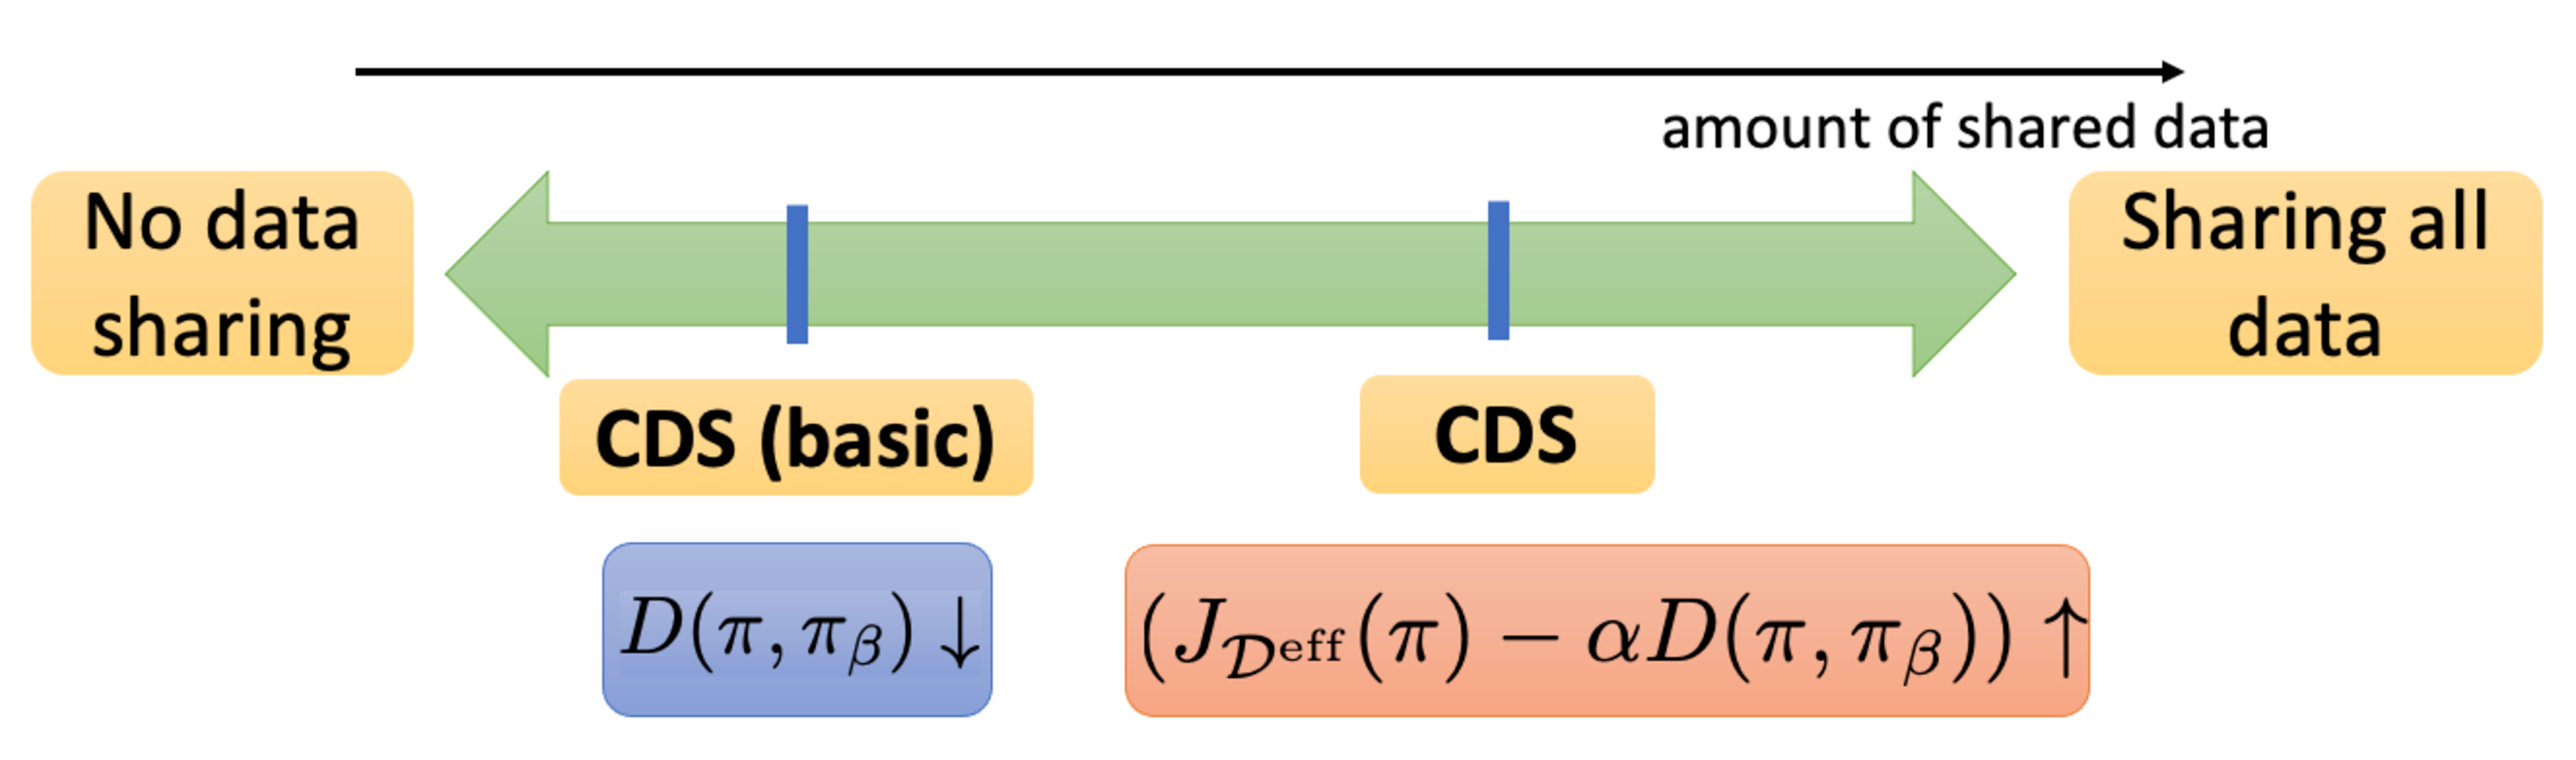
\includegraphics[width=0.99\linewidth]{chapters/cds/cds_variants.pdf}
%%CF.8.1: I think this is a nice figure. My only comment is that it isn't clear what "naive data sharing" means without having read parts of the main text. (and you should expect readers to skim figures without reading all of the text. I would change it to something like "Sharing all data" instead.
\vspace{-0.6cm}
\caption{\label{fig:cds_variants_main} \footnotesize A schematic comparing \textbf{CDS} and \textbf{CDS (basic)} data sharing schemes relative to no sharing (left extreme) and full data sharing (right extreme). While p-CDS only shares data when distributional shift is strictly reduced, o-CDS is more optimistic and shares data when the objective in Equation~\ref{eqn:generic_multitask_offline_rl} is larger. Typically, we would expect that CDS shares more transitions than CDS (basic).}
\vspace{-0.6cm}
\end{wrapfigure}
Next, we present the complete version of our method. The complete version of CDS, which we will refer to as \textbf{CDS}, for notational brevity is derived from the following perspective: we note that a data sharing scheme can be viewed as altering the dataset $\mathcal{D}^\mathrm{eff}_i$, and hence the effective behavior policy, $\pi^\mathrm{eff}_\beta(\mathbf{a}|\bs, i)$.
Thus, we can directly \emph{optimize} the objective in Equation~\ref{eqn:generic_multitask_offline_rl} with respect to $\pi^\mathrm{eff}_\beta$,
in addition to $\pi$, where $\pi^\mathrm{eff}_\beta$ belongs to the set of all possible effective behavior policies that can be obtained via any form of data sharing. Note that unlike CDS (basic), this approach would not rely on only indirectly controlling the objective in Equation~\ref{eqn:generic_multitask_offline_rl} by controlling distributional shift, but would aim to directly optimize the objective in Equation~\ref{eqn:generic_multitask_offline_rl}.  We formalize this optimization below in Equation~\ref{eqn:optimize_behavior}:
\begin{align}
\label{eqn:optimize_behavior}
    % &(\pi^*(\cdot|\cdot, i), \pi^\mathrm{eff}_\beta(\cdot|\cdot, i))\nonumber\\
    \arg \max_{\pi} \textcolor{red}{\max_{\pi^\mathrm{eff}_\beta \in \Pi_{\mathrm{relabel}}}}~~~ \left[J_{\mathcal{D}^\mathrm{eff}_i}(\pi) - \alpha D(\pi, \pi^\mathrm{eff}_\beta; i)\right],
\end{align}
where $\Pi_{\mathrm{relabel}}$ denotes the set of all possible behavior policies that can be obtained via relabeling. The next result characterizes safe policy improvement for Equation~\ref{eqn:optimize_behavior} and discusses how it leads to improvement over the behavior policy and also produces an effective practical method.
\begin{proposition}[Characterizing safe-policy improvement for CDS.] 
\label{prop:spi_thm}
Let $\pi^*(\mathbf{a}|\bs)$ be the policy obtained by optimizing Equation~\ref{eqn:optimize_behavior}, and let $\pi_\beta(\mathbf{a}|\bs)$ be the behavior policy for $\mathcal{D}_i$. Then, w.h.p. $\geq 1 - \delta$, $\pi^*$ is a $\zeta$-safe policy improvement over $\pi_\beta$, i.e., $J(\pi^*) \geq J(\pi_\beta) - \zeta$, where $\zeta$ is given by:
\begin{align*}
\small{
    \zeta = \mathcal{O}\left(\frac{1}{(1 - \gamma)^2}\right)  \mathbb{E}_{\bs \sim d^{\pi^*}_{\mathcal{D}^\mathrm{eff}_i}}\left[\sqrt{\frac{D_{\text{CQL}}(\pi^*, \pi_\beta^*)(\bs) + 1}{|\mathcal{D}^\mathrm{eff}_i(\bs)|}} \right]
    -  \left[\alpha D(\pi^*, \pi_\beta^*) + \underbrace{J(\pi^*_\beta) - J(\pi_\beta)}_{\text{(a)}} \right],}
\end{align*}
where $\mathcal{D}^\mathrm{eff}_i \sim d^{\pi_\beta^*}(\bs)$ and $\pi^*_\beta(\mathbf{a}|\bs)$ denotes the policy $\pi \in \Pi_{\text{relabel}}$ that maximizes Equation~\ref{eqn:optimize_behavior}. 
\end{proposition}
%%CF.8.1: I might consider putting this theoretical result back to the appendix. Right now, the main method doesn't come until the bottom of page 7, and the practical implementation doesn't come until page 8. Given that you can only really expect the reader to read ~9 pages, I think that the core info about the method is more important than this theoretical result.

A proof and analysis of this proposition is provided in Appendix~\ref{app:proofs},
%%SL.8.1: "Using simple arguments" kind of carries no information, though if we can (very) briefly summarize the argument, that could be nice
%%CF.8.1: +1. It's also a bad idea to suggest to the reader that something is obvious/trivial because it might not be obvious to them, and this is what you seem to be suggesting here (though to a lesser extent)
where we note that the bound in Proposition~\ref{prop:spi_thm} is stronger than both no data sharing as well as na\"ive data sharing. We show in Appendix~\ref{app:proofs} that optimizing Equation~\ref{eqn:optimize_behavior} reduces the numerator $D_\mathrm{CQL}(\pi^*, \pi_\beta^*)$ term while also increasing $|\mathcal{D}^\mathrm{eff}_i(\bs)|$, thus reducing the amount of sampling error. In addition, Lemma~\ref{lemma:a_gt_0} shows that the improvement term $(a)$ is guaranteed to be positive if a large enough $\alpha$ is chosen in Equation~\ref{eqn:optimize_behavior}. Combining these, we find data sharing using Equation~\ref{eqn:optimize_behavior} improves over both complete data sharing (which may increase $D_\mathrm{CQL}(\pi, \pi_\beta)$) and no data sharing (which does not increase $|\mathcal{D}^\mathrm{eff}_i(\bs)|$). A schematic comparing the two variants of CDS and na\"ive and no data sharing schemes is shown in Figure~\ref{fig:cds_variants_main}.



{\textbf{Optimizing Equation~\ref{eqn:optimize_behavior} tractably.}} 
%%CF.8.1: I'm not sure if you need the underline in addition to the bolded paragraph header.
The next step is to effectively convert Equation~\ref{eqn:optimize_behavior} into a simple condition for data sharing in  multi-task offline RL. While directly solving Equation~\ref{eqn:optimize_behavior} is intractable in practice, since both the terms depend on $\pi^\mathrm{eff}_\beta(\mathbf{a}|\bs)$ (since the first term $J_{\mathcal{D}^\mathrm{eff}}(\pi)$ depends on the empirical MDP induced by the effective behavior policy and the amount of sampling error), we need to instead  solve Equation~\ref{eqn:optimize_behavior} approximately. Fortunately, we can optimize a \textit{lower-bound approximation} to Equation~\ref{eqn:optimize_behavior} that uses the dataset state distribution for the policy update in Equation~\ref{eqn:optimize_behavior} similar to modern actor-critic methods~\citep{degris2012off,lillicrap2015continuous,fujimoto2018addressing,haarnoja2018soft,kumar2020conservative} which only introduces an additional $D(\pi, \pi_\beta)$ term in the objective. This objective is given by: $\mathbb{E}_{\bs \sim \mathcal{D}^{\mathrm{eff}}_i}[\mathbb{E}_\pi[Q(\bs, \mathbf{a}, i)] - \alpha' D(\pi(\cdot|\bs,i), \pi_\beta^\mathrm{eff}(\cdot|\bs,i))]$, which is equal to the expected ``conservative Q-value'' $\hat{Q}^\pi(\bs, \mathbf{a}, i)$ on dataset states, policy actions and task $i$. Optimizing this objective via a co-ordinate descent on $\pi$ and $\pi^\mathrm{eff}_\beta$ dictates that $\pi$ be updated using a standard update of maximizing the conservative Q-function, $\hat{Q}^\pi$ (equal to the difference of the Q-function and $D(\pi, \pi^{\mathrm{eff}}_\beta; i)$).
Moreover, $\pi^{\mathrm{eff}}_\beta$ should also be updated towards maximizing the same expectation, $\mathbb{E}_{\bs, \mathbf{a} \sim \mathcal{D}^\mathrm{eff}_i}[\hat{Q}^\pi(\bs, \mathbf{a}, i)] := \mathbb{E}_{\bs, \mathbf{a} \sim \mathcal{D}^\mathrm{eff}_i}[Q(\bs, \mathbf{a}, i)] - \alpha D(\pi, \pi_\beta^\mathrm{eff}; i)$. This implies that when updating the behavior policy during relabeling, we should prefer state-action pairs that maximize the conservative Q-function.
% Additionally $\pi^{\mathrm{eff}}_\beta$ should be updated towards minimizing the distribution shift $\mathbb{E}_{\bs, \mathbf{a} \sim \mathcal{D}^\mathrm{eff}_i}[ D(\pi, \pi_\beta^\mathrm{eff}; i)]$, i.e. learning a new behavior policy of task $i$ with minimal distribution shift after relabeling. In the case where $D(\pi, \pi_\beta^\mathrm{eff}; i) = D_\text{CQL}(\pi, \pi_\beta^\mathrm{eff}; i)$, we have the following objective for updating $\pi_\beta$: $\min_{\pi_\beta}\mathbb{E}_{\bs, \mathbf{a} \sim \mathcal{D}^\mathrm{eff}_i}[\hat{Q}^\pi(\bs,\mathbf{a}, i)]$
% \begin{align}
%     J_{\mathcal{D}^\mathrm{eff}_i}(\pi) - \alpha D(\pi, \pi^\mathrm{eff}_\beta; i) &:= \mathbb{E}_{\bs, \mathbf{a} \sim d^\pi_{\mathrm{eff}}}\left[Q(\bs, \mathbf{a}) - \alpha D(\pi, \pi_\right] 
% \end{align}


\textbf{{Deriving the data sharing strategy for CDS.}}
%%SL.8.1: not clear what the word "condition" means
%%CF.8.1: +1. What condition are you deriving?
%%AK: fixed
Utilizing the insights for optimizing Equation~\ref{eqn:optimize_behavior} tractably as discussed above, we now present the effective data sharing rule prescribed by CDS. For any given task $i$, we want relabeling to incorporate transitions with the highest conservative Q-value into the resulting dataset $\mathcal{D}^\mathrm{eff}_i$, as this will directly optimize the tractable lower bound on Equation~\ref{eqn:optimize_behavior}. While directly optimizing Equation~\ref{eqn:optimize_behavior} will enjoy benefits of reduced sampling error since $J_{\mathcal{D}^\mathrm{eff}_i}(\pi)$ also depends on sampling error, our tractable lower bound approximation does not enjoy this benefit. This is because optimizing the lower-bound only increases the frequency of a state in the dataset, $|\mathcal{D}^\mathrm{eff}_i(\bs)|$ by atmost 1. To encourage further reduction in sampling error, we modify CDS to instead share all transitions with a conservative Q-value more than the top $k^\text{th}$ quantile of the original dataset $\mathcal{D}_i$, where $k$ is a hyperparameter. This provably increases the objective value in Equation~\ref{eqn:optimize_behavior} still ensuring that term $(a) > 0$ in Proposition~\ref{prop:spi_thm}, while also reducing $|\mathcal{D}^{\mathrm{eff}}_i(\bs)|$ in the denominator. Thus, for a given transition $(\bs, \mathbf{a}, \bs') \in \mathcal{D}_j$,  
\begin{tcolorbox}[colback=blue!6!white,colframe=black,boxsep=0pt,top=-5pt,bottom=5pt]
\begin{align}
   \text{\textbf{CDS}:~~~~~~~~} \!\!\!\!\!\!\!\!\!(\bs, \mathbf{a}, r_i, \bs') \in \mathcal{D}^{\mathrm{eff}}_i  \text{~if~} {\Delta}^\pi(\bs, \mathbf{a})\! := \hat{Q}^\pi(\bs, \mathbf{a}, i) - P_{k\%}\!\left\{\!\hat{Q}^\pi(\bs', \mathbf{a}', i)\!\!: \bs', \mathbf{a}' \sim \mathcal{D}_i\!\right\} \geq 0,
\label{eqn:method}
\end{align}
\end{tcolorbox}
%%AK: is it obvious that z^k denotes the k0th quantile? What other standard notations are used for quantiles?
%%TY.8.2: I think it's P_k%. I rewrote it.
where $\hat{Q}^\pi$ denotes the learned conservative Q-function estimate. If the condition in Equation~\ref{eqn:method} holds for the given $(\bs, \mathbf{a})$, then the corresponding relabeled transition, $(\bs, \mathbf{a}, r_{i}(\bs, \mathbf{a}), \bs')$ is added to $\mathcal{D}^\mathrm{eff}_i$. 

We summarize the pesudocode of CDS in Algorithm~\ref{alg:cds} in Appendix~\ref{app:alg} and include the practical implementation details of CDS in Appendix~\ref{app:details}.

% Our main data-sharing scheme, o-\cdsmethodname, is based on the insight discussed above. o-\cdsmethodname\ first runs any standard conservative offline RL algorithm on each task individually without any data sharing. Consistent with our insight from above, relabeling a transition that contributes a lower conservative Q-value to the current task will only decrease the average conservative Q-value of the effective resulting dataset for this task, whereas the $\pi^\mathrm{eff}_\beta$ is to be optimized to maximize this value. On the other hand, more samples in $\mathcal{D}^\mathrm{eff}_i$ will reduce sampling error. Hence, we employ a simple rule to decide which transitions from the data for other tasks will be relabeled to the current task, say task $i$: o-\cdsmethodname\ checks if the conservative Q-value estimate for this transition under task $i$ is greater than a specific percentile of the conservative Q-value for the original dataset for task $i$, $\mathcal{D}_i$. This is sufficient to increase the average conservative Q-value in $\mathcal{D}^\mathrm{eff}_i$ after relabeling, while still allowing us to keep sampling error under control.

% Thus, o-\cdsmethodname\ first estimates a conservative Q-value estimate, $\hat{Q}^\pi(\bs, \mathbf{a}, i)$ (which can be obtained via any offline RL algorithm), and for a given transition, $(\bs, \mathbf{a}, r_j, \bs') \in \mathcal{D}_j$ it then checks if the following condition is satisfied: 

% If the condition in Equation~\ref{eqn:method} holds for the given $(\bs, \mathbf{a})$, then the corresponding relabeled transition, $(\bs, \mathbf{a}, r_{i}(\bs, \mathbf{a}), \bs')$ is added to $\mathcal{D}^\mathrm{eff}_i$. \arxiv{In practice, instead of computing $\mathbb{E}_{\bs', \mathbf{a}' \sim \mathcal{D}_i}\left[ \hat{Q}^\pi(\bs', \mathbf{a}', i) \right]$, we use the $90$-th percentile of $\hat{Q}^\pi(\bs', \mathbf{a}', i)$ $\forall \bs', \mathbf{a}' \in \mathcal{D}_i$.} This rule for relabeling is applied independently on each transition $(\bs, \mathbf{a}, r, \bs') \in \mathcal{D}$. 

% \subsection{{Practical implementation of \cdsmethodname}} 
%%CF.8.1: In the section header and throughout the section, I would just have this discuss the main variant, not both. 
% The pseudocode of CDS is summarized in Algorithm~\ref{alg:cds} in Appendix~\ref{app:alg}. The complete variant of CDS can be directly implemented using the rule in Equation~\ref{eqn:method} with conservative Q-value estimates obtained via any offline RL method that constrains the learned policy to the behavior policy. For implementing \cdsmethodname\ (basic), we reparameterize the divergence $D$ in Equation~\ref{eqn:pessimistically_conservative} to use the learned conservative Q-values. This is especially useful for our implementation since we utilize CQL as the base offline RL method, and hence we do not have access to an explicit divergence. In this case, $\Delta^\pi(\bs, \mathbf{a})$ can be redefined as, $\Delta^\pi(\bs, \mathbf{a}) :=$
% \begin{align}
%     \mathbb{E}_{\bs' \sim \mathcal{D}^i}\left[\mathbb{E}_{\mathbf{a}' \sim \pi}[\hat{Q}(\bs', \mathbf{a}', i)] - \mathbb{E}_{\mathbf{a}'' \sim \mathcal{D}_i}[\hat{Q}(\bs', \mathbf{a}'', i)]\right] - \left(\mathbb{E}_{\mathbf{a}' \sim \pi}[\hat{Q}(\bs, \mathbf{a}', i)] - Q(\bs, \mathbf{a}, i)\right),
% \label{eqn:p-cds}
% \end{align}
% % \begin{align}
% %     \Delta^\pi(\bs, \mathbf{a})  := 
% %     -\left(\mathbb{E}_{\mathbf{a} \sim \mu(\cdot|\bs)}\!\left[Q(\bs,\mathbf{a}, i)\right]\!-\!\mathbb{E}_{\bs', \mathbf{a}' \sim \mathcal{D}_i}\!\left[Q(\bs',\mathbf{a}', i)\right]\right) +
% %     \left(\mathbb{E}_{\bs\sim \mathcal{D}_i, \mathbf{a} \sim \mu(\cdot|\bs)}\!\left[Q(\bs,\mathbf{a}, i)\right]\!-\!\mathbb{E}_{\bs', \mathbf{a}' \sim \mathcal{D}_i}\!\left[Q(\bs',\mathbf{a}', i)\right]\right)
% % \label{eqn:p-cds}
% % \end{align}
% % where $\mu(\cdot|s)$ is a wide sampling distribution such as the uniform distribution over the range of actions.
% Equation~\ref{eqn:p-cds} can be viewed as the difference between the CQL~\citep{kumar2020conservative} regularization term on a given $(\bs, \mathbf{a})$ and the original dataset for task $i$, $\mathcal{D}_i$. This CQL regularization term is equal to the divergence between the learned policy $\pi(\cdot|\bs)$ and the behavior policy $\pi_\beta(\cdot|\bs)$, therefore Equation~\ref{eqn:p-cds} practically computes Equation~\ref{eqn:pessimistically_conservative}. 
% % Intuitively, if the condition in Equation~\ref{eqn:p-cds} is true for certain $(\bs, \mathbf{a})$, adding it to $\mathcal{D}^\mathrm{eff}_i$ would decrease the expected CQL regularization term, which estimates the distributional shift $D_\text{CQL}(\pi(\cdot|\cdot, i), \pi_\beta^{\text{eff}}(\cdot|\cdot, i))$.

% Finally, both variants of \cdsmethodname\ train a policy, 
% $\pi(\mathbf{a}|\bs; i)$, either conditioned on the task $i$ (i.e., with weight sharing) or a separate $\pi(\mathbf{a}|\bs)$ policy for each task with no weight sharing, using the resulting relabeled dataset, $\mathcal{D}^\mathrm{eff}_i$.
% For practical implementation details of \cdsmethodname\, see Appendix~\ref{app:details}.

%%CF.5.22: you seem to have forgotten the punch line here.

%%SL.5.23: I think it would really help to add some pseudocode that describes the method. Right now, readers have to do a bit of detective work to piece together the complete algorithm. Pseudocode + algorithm summary would really help.

%%AK: just regular CQL weighted by the weights w_(s, a) described above

%%AK: there is a critical point here -- if we keep doing our scheme continually, would we eventually diverge, since we are doing many rounds of relabelling effectively? How should we handle that?



%% Theoretical Analysis